\begin{figure}[tb]
    \centering
    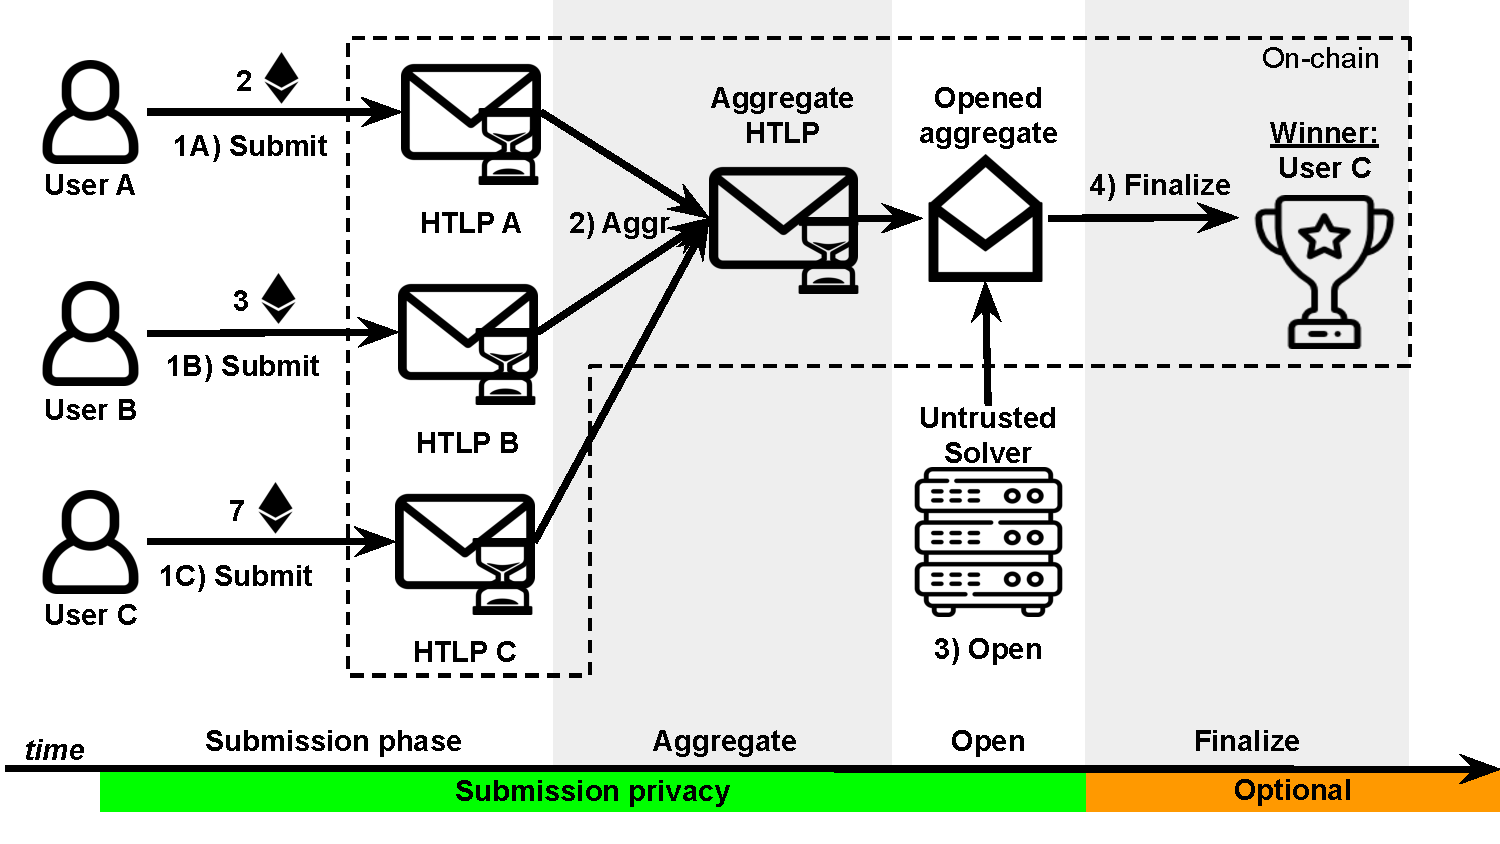
\includegraphics[width=0.95\textwidth]{cicada/figs/cicada-explainer.pdf}
    \caption{The system model of Cicada. \emph{(1) Submission phase:} users generate their bids/ballots as HTLPs and post them to a public bulletin board, e.g., a blockchain. \emph{(2) Aggregation:} an on-chain contract homomorphically combines submissions into an aggregate puzzle as they are submitted. \emph{(3) Opening:} after all submissions have been aggregated, an off-chain entity solves the aggregate HTLP using $\Ttime$ sequential steps and submits the solution to the contract. \emph{(4) Finalize:} The smart contract may do some final computation over the solution to compute the result and announces the winner. Submission privacy is ensured only until the start of the $\mathsf{Open}$ phase. 
    In \Cref{sec:everlasting_ballot_privacy}, we show how voters can pool their submissions to achieve everlasting ballot privacy.
    }
    \label{fig:cicada-explainer}
\end{figure}
